\subsection{Yeast and primate datasets}\label{sec:results:small}

All 30 DistributedPanGA runs produced output byte-identical to FastGA's.
Table~\ref{tab:pipeline} gives the time of each stage and the total for
every configuration.

\begin{table}[htbp]
\caption{DistributedPanGA time per stage, in seconds. ``Seeds'' is seed
generation and redistribution; ``Alignment'' includes PAF output.
``Total'' is the sum of the four stages. Each row is the run with the
median total time of three.}\label{tab:pipeline}
\begin{tabular}{@{}lrrrrrrr@{}}
\toprule
Dataset & Nodes & Ranks & Extraction & Sort & Seeds & Alignment & Total \\
\midrule
\csname @@input\endcsname fig/table_pipeline.tex
\botrule
\end{tabular}
\end{table}

\begin{figure}[htbp]
\centering
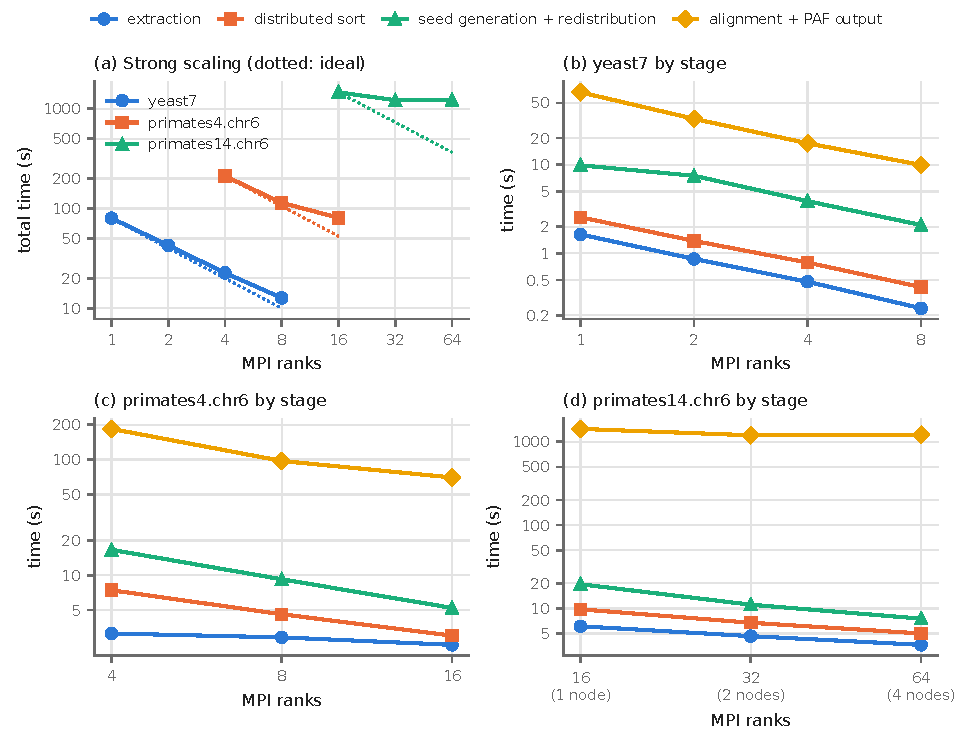
\includegraphics[width=\textwidth]{fig/strong_scaling.pdf}
\caption{All panels use log--log axes. (a) Total time against ranks. yeast7 and primates4.chr6 run on one
node. primates14.chr6 uses 16 ranks per node (1, 2 and 4 nodes). Dotted lines
show ideal scaling from the smallest run. (b)--(d) Time per stage for each
dataset; the legend at the top applies to these panels.}\label{fig:strong}
\end{figure}

\paragraph{Strong scaling on one node.} From 1 to 8 ranks, yeast7 drops
from 79.97\,s to 12.69\,s, a speedup of 6.3 (79\% parallel efficiency;
Fig.~\ref{fig:strong}a). From 4 to 16 ranks, primates4.chr6 drops from
211.47\,s to 80.76\,s, a speedup of 2.6 (65\%). Alignment takes 77--87\% of
the total time in these runs.

\paragraph{Strong scaling across nodes.} With 16 ranks per node,
primates14.chr6 takes 1,463.94\,s on one node, 1,218.54\,s on two and
1,229.09\,s on four. Alignment takes 98--99\% of the total time and stays between
1,196.09\,s and 1,428.58\,s (Fig.~\ref{fig:strong}d). From 16 to 64 ranks,
extraction falls from 6.10\,s to 3.65\,s, the sort from 9.76\,s to 5.00\,s,
and seed generation and redistribution from 19.50\,s to 7.53\,s.

Table~\ref{tab:perrank} breaks the alignment stage down by rank. From 16 to
64 ranks on primates14.chr6, the average rank's alignment time falls from
722.15\,s to 183.43\,s, while the slowest rank's stays between 1,169.50\,s
and 1,393.88\,s. At 64 ranks the slowest rank takes 6.59 times the
average; on primates4.chr6 the ratio grows from 1.09 at 4 ranks to 1.70 at
16.

\begin{table}[htbp]
\caption{Alignment time per rank, in seconds, for the runs in
Table~\ref{tab:pipeline}: the slowest, average and fastest rank, and the
slowest divided by the average. Alignment time here is the time spent
aligning seed chains, without sorting seeds or writing PAF.}\label{tab:perrank}
\begin{tabular}{@{}lrrrrrr@{}}
\toprule
Dataset & Nodes & Ranks & Slowest & Average & Fastest & Slowest/avg. \\
\midrule
\csname @@input\endcsname fig/table_perrank.tex
\botrule
\end{tabular}
\end{table}

\begin{figure}[htbp]
\centering
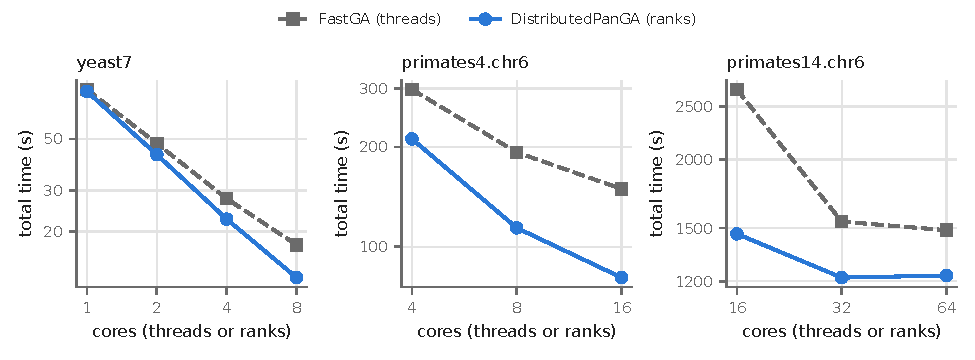
\includegraphics[width=\textwidth]{fig/vs_fastga.pdf}
\caption{DistributedPanGA ($P$ ranks) against FastGA ($t$ threads on one
node) at equal core counts, on log--log axes. For primates14.chr6,
DistributedPanGA uses 16 ranks per node.}\label{fig:fastga}
\end{figure}

\begin{table}[htbp]
\caption{FastGA time per step on one node, in seconds. Each row is the run
with the median total time of three. \texttt{GIXmake} builds the index,
\texttt{FastGA} aligns and \texttt{ALNtoPAF} writes PAF.}\label{tab:fastga}
\begin{tabular}{@{}lrrrrr@{}}
\toprule
Dataset & Threads & \texttt{GIXmake} & \texttt{FastGA} & \texttt{ALNtoPAF} & Total \\
\midrule
\csname @@input\endcsname fig/table_fastga.tex
\botrule
\end{tabular}
\end{table}

\paragraph{Comparison with FastGA.} Table~\ref{tab:fastga} gives FastGA's time per step. All FastGA runs produced the same
alignments as the reference. At equal core counts, DistributedPanGA is
1.0--1.4$\times$ faster than FastGA on yeast7 (1 to 8 cores),
1.4--1.9$\times$ on primates4.chr6 (4 to 16 cores) and 1.2--1.8$\times$ on
primates14.chr6 (16 to 64 cores) (Fig.~\ref{fig:fastga}). From 4 to 16 cores
on primates4.chr6, FastGA speeds up by 2.0 and DistributedPanGA by 2.6. From
16 to 64 cores on primates14.chr6, FastGA speeds up by 1.8 and
DistributedPanGA by 1.2.

FastGA's fastest one-node time on primates14.chr6 is 1,486.52\,s, at 64
threads. DistributedPanGA takes 1,463.94\,s on one node, 1,218.54\,s on two
and 1,229.09\,s on four, 1.0, 1.2 and 1.2$\times$ faster than that time.

\paragraph{Weak scaling.} Two sets of three runs have about the same number
of bases per rank: 83\,Mbp (yeast7 on 1 rank, primates4.chr6 on 8,
primates14.chr6 on 32 over two nodes) and 42\,Mbp (2, 16 and 64 ranks).
At 83\,Mbp per rank, seed generation and redistribution take 9.87, 9.23 and
11.07\,s; extraction grows 2.9$\times$ (1.63 to 4.65\,s), the sort
2.6$\times$ (2.55 to 6.73\,s) and alignment 18$\times$ (65.92 to
1,196.09\,s).

Table~\ref{tab:weak} gives the alignment output per rank for these runs.
At 83\,Mbp per rank, from yeast7 to primates14.chr6 the aligned bases per
rank grow 7.9$\times$, the average rank's alignment time 8.6$\times$ and
the slowest rank's 28$\times$. primates4.chr6 aligns 1.07$\times$ as many
bases per rank as yeast7, in 4.5$\times$ as many alignments, and its
average rank takes 1.7$\times$ as long.

\begin{table}[htbp]
\caption{Weak scaling: alignment output and alignment time per rank. Aligned
bases are the summed lengths of all alignments in FastGA's output, which
every run reproduces, divided by the ranks; one input base is counted once
for every alignment it is part of. Alignment time is as in
Table~\ref{tab:perrank}.}\label{tab:weak}
\begin{tabular}{@{}lrrrrrr@{}}
\toprule
 & & Input & Aligned & Alignments & \multicolumn{2}{c}{Alignment time (s)} \\
\cmidrule{6-7}
Dataset & Ranks & Mbp/rank & Mbp/rank & per rank & Average & Slowest \\
\midrule
\csname @@input\endcsname fig/table_weak.tex
\botrule
\end{tabular}
\end{table}
